\documentclass[12pt]{article}

\usepackage{graphicx}
\usepackage{amsmath}
\usepackage{amssymb}
\usepackage{natbib}
\usepackage{amsfonts}
\usepackage{multicol}
\usepackage{float}
\usepackage{oldgerm}
\usepackage{bm}
\usepackage{mathtools}
\usepackage{wrapfig}
\usepackage{fancyhdr}
\usepackage[export]{adjustbox}
\usepackage{xcolor}
\usepackage[shortlabels]{enumitem}

\pagestyle{empty}

\setlength{\headsep}{0.5cm}
\setlength{\oddsidemargin}{-0.5cm}
\setlength{\textwidth}{16.5cm}
\setlength{\textheight}{24cm}
\voffset = -2cm


\pagestyle{fancy}
\fancyhf{}
\rfoot{
\includegraphics[width=1.0in]{cnm.png}}
\lfoot{ENGR2910 - Midterm 2}
\setlength\parindent{0pt}
\begin{document}

\begin{center}
\hfil
{\large\bf {ENGR 2910-101: Circuit Analysis}}
\hfill Instructor: Brian Rashap\\
Midterm 2  \hfill Due: 03/29/23\\
\hrulefill\\
\end{center}

Please show all your work and circle your answers to each question.
\newline\newline

{\bf Question 1} [25]
\newline

\begin{figure}[h!]
\centering 
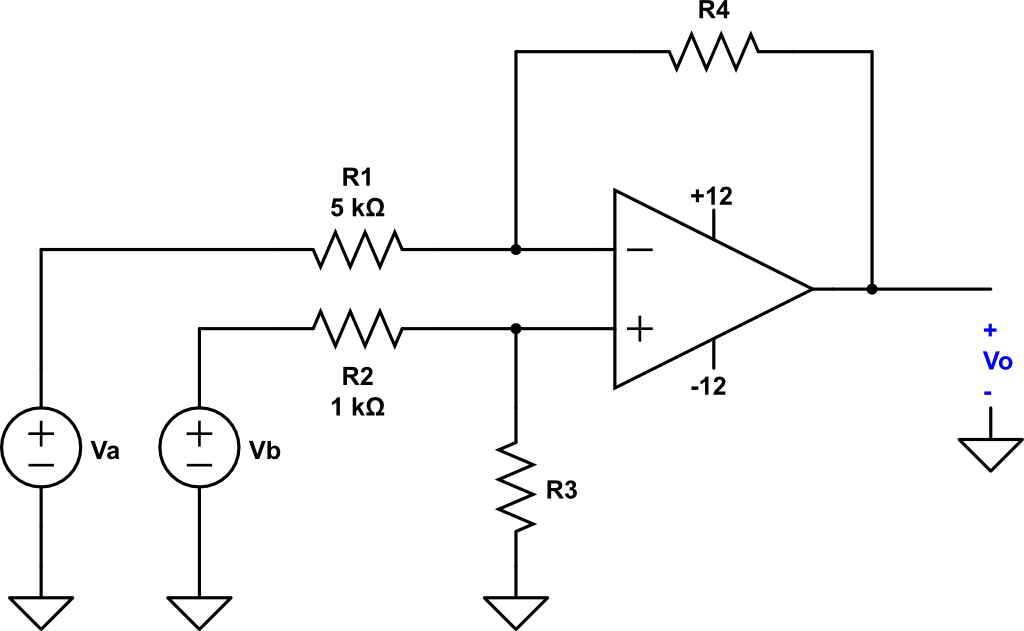
\includegraphics[clip,width=0.49\textwidth]{mid2_1.png}
\end{figure}

\begin{enumerate}[(a)]
\item For the differntial amplifier shown above, find values for $R_3$ and $R_4$ that amplify the difference between the $V_a$ and $V_b$ by 4.
\item If $V_a = 4V$, find the range for $V_b$ that keeps the amplifier in the linear operating region.
\item If the $R_1$ resistor is reduced to $4k\Omega$ and all other values remain the same, that is the new range for $V_b$ that keeps the amplifier in the linear operating region.
\item What is the $A_{dm}$, $A_{cm}$, and CMRR for the amplifier with the resistor values from (c)?
\end{enumerate}

{\bf Question 2} [25] 
\newline
What is the equivalent resistance between $A$ and $B$?

\begin{figure}[h!]
  \centering 
 \vspace{-0.1in}
 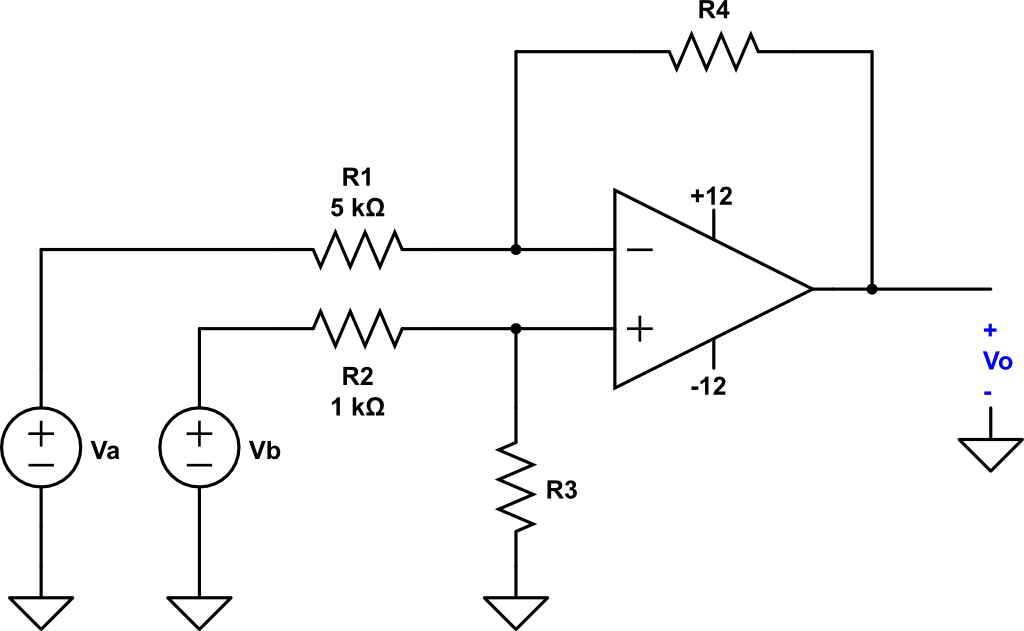
\includegraphics[clip,width=0.49\textwidth]{mid2_1.png}
\vspace{-0.1in}
\end{figure}


\newpage
{\bf Question 3} [25] 
\newline
For the below circuit has been in position a for a long time. 

\begin{figure}[h!]
     \centering
       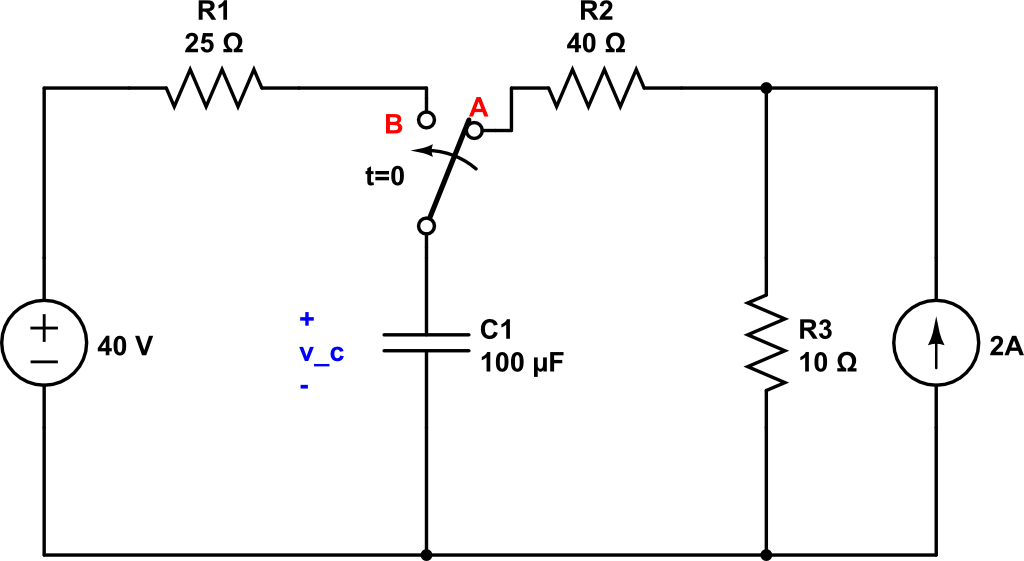
\includegraphics[clip,width=0.6\textwidth]{mid4_3.png}
\end{figure}

\begin{enumerate}[(a)]
\item At $t=0$, the switch instantly moves to position b and stays there. Find:
\begin{enumerate}[(i)]
\item The initial and final values for the capacitor voltage
\item The time constant
\item The expression for the capacitor voltage for $t \geq 0$.
\end{enumerate}
\item At time xxx the switch moves back to position a. Find
\begin{enumerate}[(i)]
\item The initial and final values for the capacitor voltage
\item The time constant
\item The expression for the capacitor voltage for $t \geq xxx$.
\end{enumerate}

\end{enumerate}

\newpage
{\bf Question 4} [25] 
\newline
Consider the voltage divider below (both with and without a load):

\begin{figure}[!h]
  \centering 
  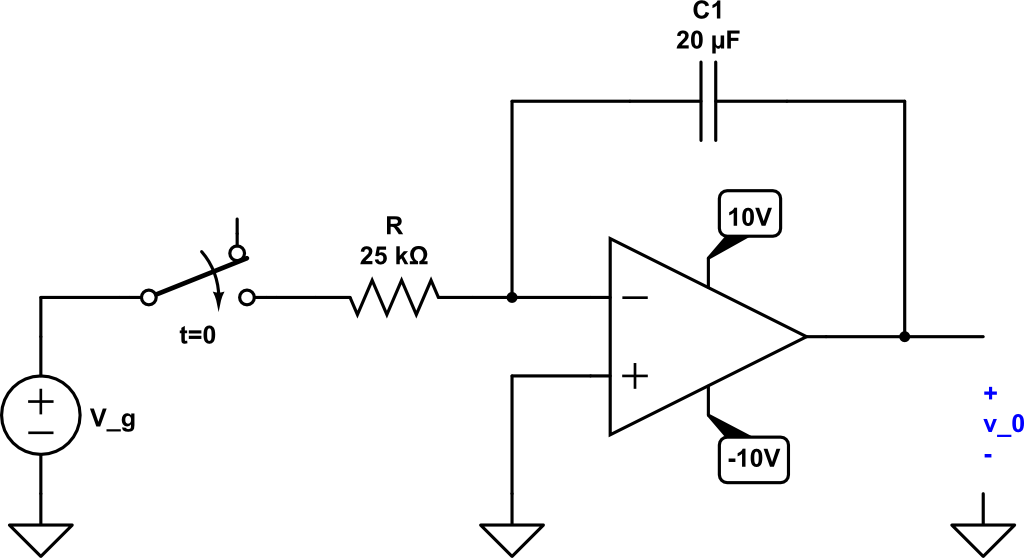
\includegraphics[clip,width=0.6\textwidth]{mid2_4.png}
\end{figure}

\begin{figure}[!h]
  \centering 
  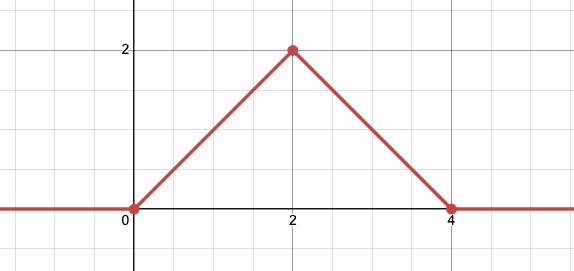
\includegraphics[clip,width=0.6\textwidth]{mid2_4a.png}
\end{figure}

\begin{enumerate}[(a)]
\item Find a numerical expression for $V_g$ for $0s \leq t \leq 2s$ and $2s \leq t \leq 4s$
\item Derive the numerical expression for $V_0$ for $0s \leq t \leq 2s$ and $2s \leq t \leq 4s$
\item Sketch the output waveform between $0s$ and $4s$.
\item Now consider a waveform with a peak at $4V$ rather than $2V$, sketch the resulting waveform.
\end{enumerate}
\newpage

\end{document}
